\section{Modelfitting framework}

In the early stages of the project it was decided that it would be necessary to create a custom application to process and display voxel data.
The rationale behind doing this instead of using an existing solution such as Matlab or Octave was threefold:

\begin{enumerate}
	\item The sample dataset from the Southampton Gait Tunnel is stored in a custom binary format, the parsing and display of which is
		undertaken by an C library, Vis4D, written by Richard Seely.
		The library is efficient and well-tested, therefore it would be beneficial to make as much use of it as possible.
	\item One of the goals of the project is to investigate ways in which the algorithms can be made parallelizable and applicable to real-time processing.
		As a prototyping language Matlab is generally less suitable for real-time or high-performance computing than a lower-level language such as C.
	\item The key aspect of this area of research that sets it aside from others in the field is that it focuses on 3D datasets.
		Visualising this 3D data in a useful way will require a custom user interface.
\end{enumerate}

It was decided to create an application that would load and process sequences of frames containing voxel data.
The application would run image-processing and classification algorithms on the data, and would be capable of handling both
the conventional and stream-processor implementations that are described throughout this chapter.

%The algorithms would be implemented as pixel-shaders, using the stream-processor capabilities of the GPU to execute code on hundreds of pixels at once.

Qt \cite{Qt} was chosen as the user-interface toolkit due to its excellent API and developer documentation.
Another advantage of using Qt is for its cross-platform compatibility - applications written using the toolkit can be compiled
for Linux, Mac OS X and Windows with no changes to the source code.
OpenGL along with the NVIDIA Cg Toolkit \cite{CgToolkit} provide a solid cross-platform foundation on which to build the shader components.

\begin{figure}[tb]
	\centering
	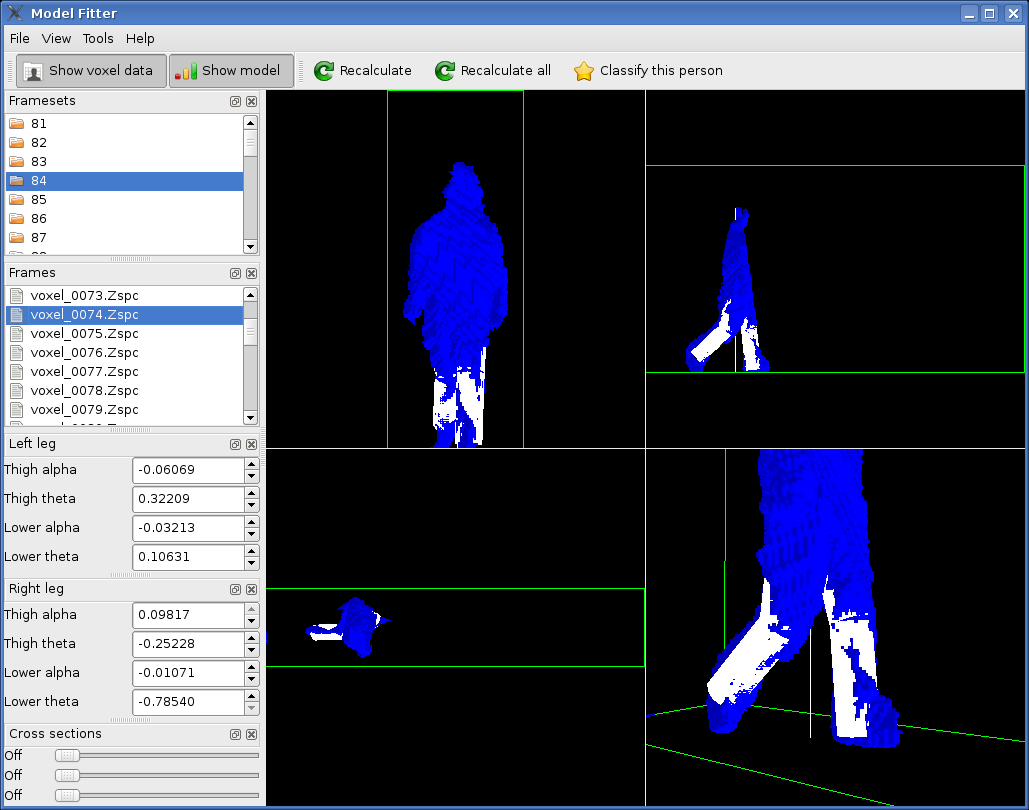
\includegraphics[height=8cm]{screenshot.png}
	\caption{Screenshot of the ``Model Fitter'' application.}
	\label{Screenshot}
\end{figure}

Figure \ref{Screenshot} shows a screenshot of the application in its completed state running under X11 on Linux.

\bigskip
The remainder of this chapter will describe the various algorithms implemented in the Model Fitter application,
and explain which of them were successful.